\subsubsection{UC 14 - Eliminare una cartella} \label{sec:UC14}
    \begin{itemize}
        \item \textbf{Attore principale}: MUA;
        \item \textbf{Descrizione}: il MUA elimina una cartella dal sistema;
        \item \textbf{Precondizioni}: il MUA sta usando la funzionalità di eliminazione di un oggetto;
        \item \textbf{Postcondizioni}: il sistema elimina la cartella con l'identificativo fornito dal MUA;
        \item \textbf{Scenario principale}:
            \begin{enumerate}
                \item il MUA invia i dettagli della cartella da eliminare al sistema (\hyperref[sec:UC14.1]{UC 14.1});
                \item il sistema elimina la cartella;
            \end{enumerate}
        \item \textbf{Inclusioni}: nessuna;
        \item \textbf{Generalizzazioni}: nessuna;
        \item \textbf{Estensioni}: nessuna.
    \end{itemize}

\begin{figure}[h]
    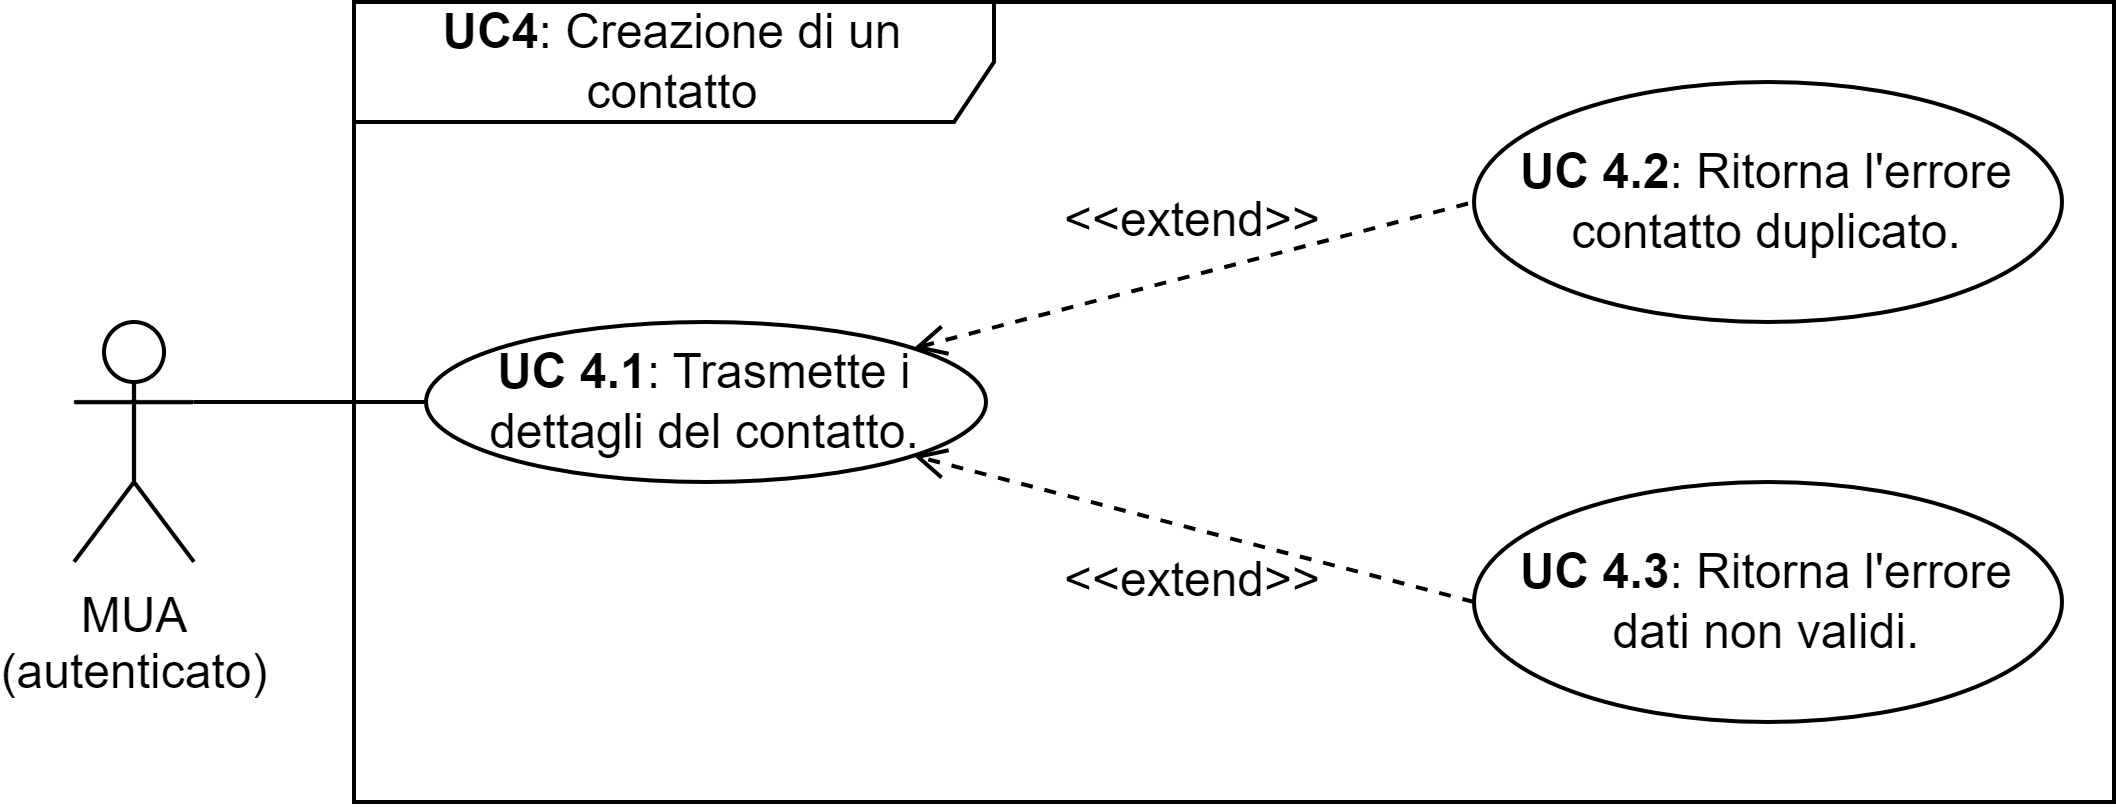
\includegraphics[width=0.85\textwidth]{sections/uc_imgs/UC04.X.png}
    \centering
    \caption{Diagramma sotto-casi UC 14.}
\end{figure}

\subsubsection{UC 14.1 - Trasmette i dettagli della cartella} \label{sec:UC14.1}
    \begin{figure}[h]
        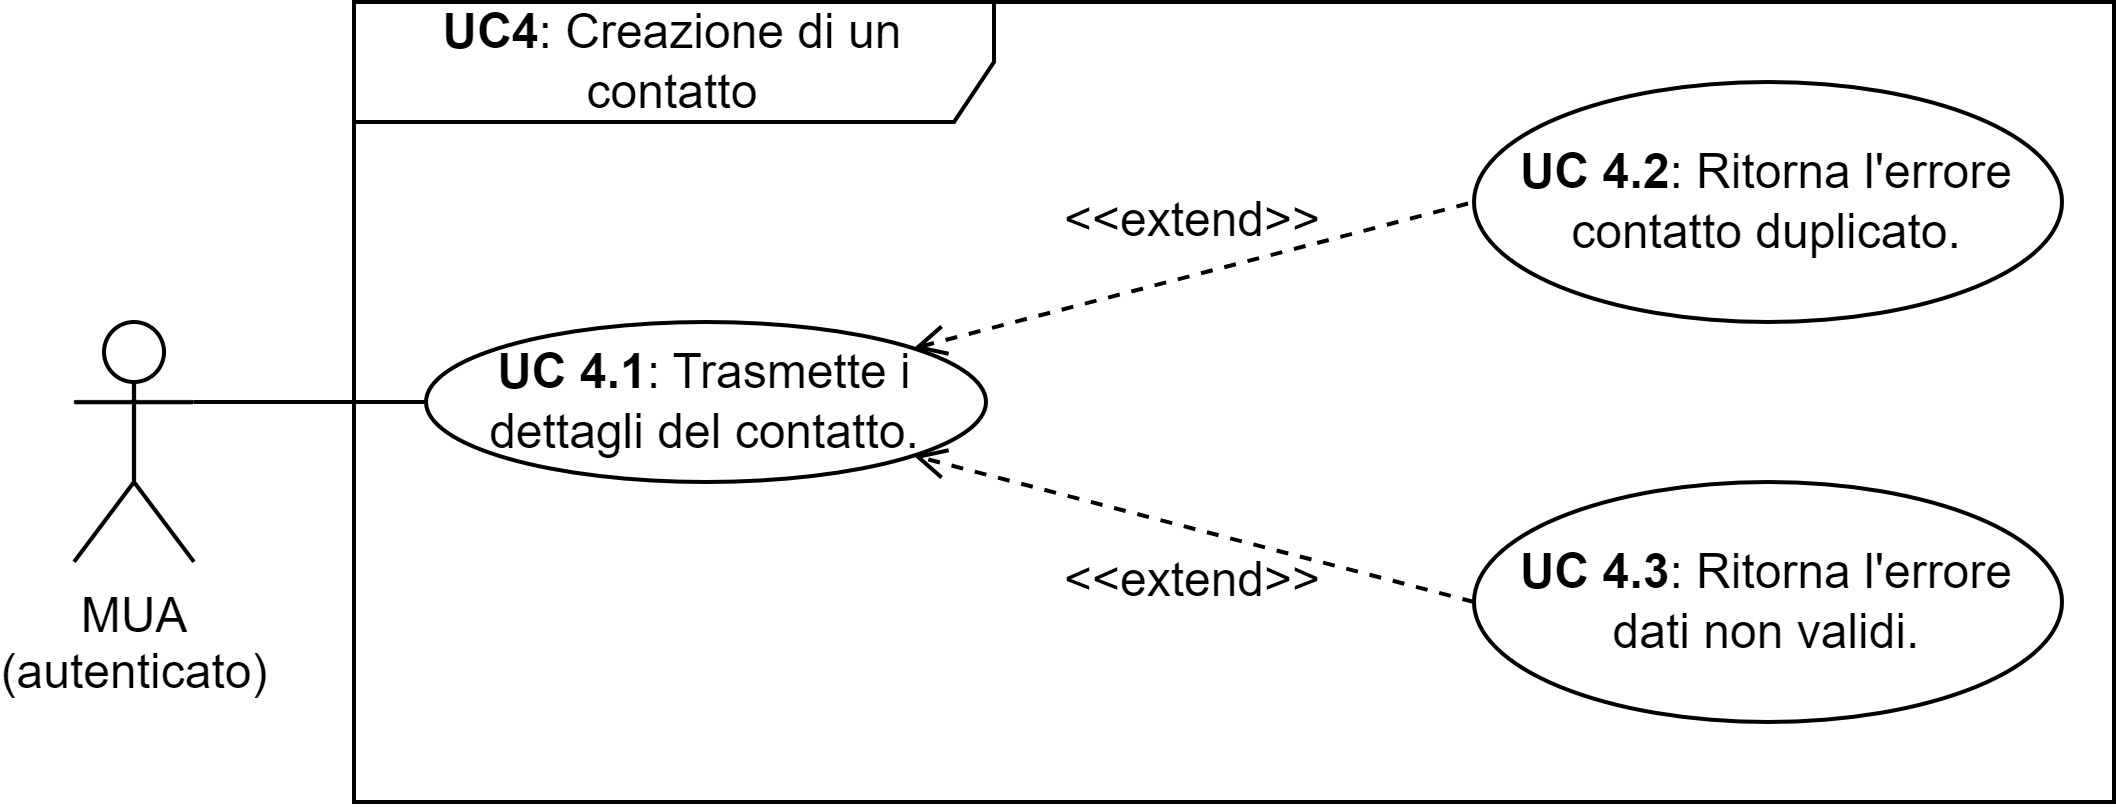
\includegraphics[width=0.85\textwidth]{sections/uc_imgs/UC04.X.png}
        \centering
        \caption{Diagramma UC 14.1.}
    \end{figure}
    \begin{itemize}
        \item \textbf{Attore principale}: MUA;
        \item \textbf{Descrizione}: il MUA invia le informazioni della cartella da eliminare al sistema;
        \item \textbf{Precondizioni}: il MUA sta usando la funzionalità di eliminazione di una cartella;
        \item \textbf{Postcondizioni}: il sistema elimina la cartella identificata dalle informazioni fornite dal MUA;
        \item \textbf{Scenario principale}:
            \begin{enumerate}
                \item il MUA invia l'identificativo della cartella al sistema;
            \end{enumerate}
        \item \textbf{Inclusioni}: nessuna;
        \item \textbf{Generalizzazioni}: nessuna;
        \item \textbf{Estensioni}:
            \begin{enumerate}[label=\alph*.]
                \item il sistema non riesce a eliminare la cartella perché non è stato trovato:
                \begin{enumerate}[label=\arabic*.]
                    \item il sistema ritorna un errore al MUA di identificativo non valido (\hyperref[sec:UC11.2]{UC 11.2}).
                \end{enumerate}
            \end{enumerate}
    \end{itemize}


\subsubsection{UC 14.2 - Ricezione errore identificativo cartella non valida} \label{sec:UC11.2}
    \begin{itemize}
        \item \textbf{Attore principale}: MUA;
        \item \textbf{Descrizione}: il sistema non riesce a eliminare la cartella perché l'identificativo cartella non è stato trovato;
        \item \textbf{Precondizioni}: il MUA sta usando la funzionalità d'invio dei dettagli al sistema di una cartella;
        \item \textbf{Postcondizioni}: il sistema non elimina la cartella, il MUA è stato notificato dell'errore;
        \item \textbf{Scenario principale}:
            \begin{enumerate}
                \item il sistema non trova la cartella con l'identificativo fornito dal MUA;
                \item il sistema non elimina la cartella e notifica il MUA dell'errore;
            \end{enumerate}
        \item \textbf{Inclusioni}: nessuna;
        \item \textbf{Generalizzazioni}: nessuna;
        \item \textbf{Estensioni}: nessuna.
    \end{itemize}
   
   
    \paragraph{UC Errore cartella contenente email} \label{sec: UC 11.4.2.1}
        \begin{itemize}
                \item Attore: MUA;
                \item Descrizione: il MUA deve ricevere un messaggio di errore adeguato quando l'eliminazione di una cartella non è andata a buon fine a causa di una o più email presenti all'interno di quella cartella;
         \item Scenario:
         \begin{enumerate}
         \item il MUA riceve il messaggio di errore;
         \end{enumerate}   
         \item Precondizioni: 
         \begin{enumerate}
             \item il MUA ha trasmesso i dati per l'emilinazione di una cartella ;
             \item la cartella contiene una o più email;
         \end{enumerate}
         \item Postcondizioni: il MUA ha ricevuto un messaggio di errore.
     \end{itemize}
     
     %eliminazione cartella con cartelle
     \paragraph{UC Errore cartella contenente cartelle} \label{sec: UC 11.4.2.1}
     \begin{itemize}
         \item Attore: MUA;
         \item Descrizione: il MUA deve ricevere un messaggio di errore adeguato quando l'eliminazione di una cartella non è andata a buon fine a causa di una o più cartelle presenti all'interno di quella cartella;
         \item Scenario:
         \begin{enumerate}
         \item il MUA riceve il messaggio di errore;
         \end{enumerate}   
         \item Precondizioni: 
         \begin{enumerate}
             \item il MUA ha trasmesso i dati per l'emilinazione di una cartella ;
             \item la cartella contiene una o più cartelle;
         \end{enumerate}
         \item Postcondizioni: il MUA ha ricevuto un messaggio di errore.
     \end{itemize}
